%%%%%%%%%%%%%%%%%%%%%%%%%%%%%%%%%%%%%%%%%
% FRI Data Science_report LaTeX Template
% Version 1.0 (28/1/2020)
% 
% Jure Demšar (jure.demsar@fri.uni-lj.si)
%
% Based on MicromouseSymp article template by:
% Mathias Legrand (legrand.mathias@gmail.com) 
% With extensive modifications by:
% Antonio Valente (antonio.luis.valente@gmail.com)
%
% License:
% CC BY-NC-SA 3.0 (http://creativecommons.org/licenses/by-nc-sa/3.0/)
%
%%%%%%%%%%%%%%%%%%%%%%%%%%%%%%%%%%%%%%%%%


%----------------------------------------------------------------------------------------
%	PACKAGES AND OTHER DOCUMENT CONFIGURATIONS
%----------------------------------------------------------------------------------------
\documentclass[fleqn,moreauthors,10pt]{ds_report}
\usepackage[english]{babel}

\graphicspath{{fig/}}




%----------------------------------------------------------------------------------------
%	ARTICLE INFORMATION
%----------------------------------------------------------------------------------------

% Header
\JournalInfo{FRI Natural language processing course 2024}

% Interim or final report
\Archive{Project report} 
%\Archive{Final report} 

% Article title
\PaperTitle{Unsupervised Domain adaptation for Sentence Classification} 

% Authors (student competitors) and their info
\Authors{Veronika Matek, Karmen Frank, and Luka Mihelič}

% Advisors
\affiliation{\textit{Advisors: Slavko Žitnik, Aleš Žagar, Boshko Koloski}}

% Keywords
\Keywords{Domain Adaptation, TSDAE, GPL, SBERT, Sentence Classification}
\newcommand{\keywordname}{Keywords}


%----------------------------------------------------------------------------------------
%	ABSTRACT
%----------------------------------------------------------------------------------------

\Abstract{
The abstract goes here. The abstract goes here. The abstract goes here. The abstract goes here. The abstract goes here. The abstract goes here. The abstract goes here. The abstract goes here. The abstract goes here. The abstract goes here. The abstract goes here. The abstract goes here. The abstract goes here. The abstract goes here. The abstract goes here. The abstract goes here. The abstract goes here. The abstract goes here. The abstract goes here. The abstract goes here. The abstract goes here. The abstract goes here. The abstract goes here. The abstract goes here. The abstract goes here. The abstract goes here.
}

%----------------------------------------------------------------------------------------

\begin{document}

% Makes all text pages the same height
\flushbottom 

% Print the title and abstract box
\maketitle 

% Removes page numbering from the first page
\thispagestyle{empty} 

%----------------------------------------------------------------------------------------
%	ARTICLE CONTENTS
%----------------------------------------------------------------------------------------

\section*{Introduction}
	Uvodni zapis - slabosti SBERT-a in podobnih metod, zakaj se uporablja TSDAE in GPL (v povezavi s prilagoditvijo domene). Osredotočili se bomo na "domain adaptation" za slovenski jezik, pri čemer bomo metode testirali nad problemom "sentimental analysis" (nekako povežemo besedilo na problem klasifikacija pri čustvih). Cilj projekta je bila implementacija metod TSDAE, GPL, s katerimi finetunamo SBERT (BERT+pooling), in testiranje metod ter primerjava rezultatov nad problemom klasifikacije stavkov v eno izmed "pos", "neg", "neutral". Opazovali smo tudi izbrane parametre tekom učenja posameznega pristopa.

	In the Introduction section you should write about the
	relevance of your work (what is the purpose of the project,
	what will we solve) and about related work (what solutions
	for the problem already exist). Where appropriate, reference
	scientific work conducted by other researchers.


%------------------------------------------------


\section*{Methods}


Use the Methods section to describe what you did an how you did it -- in what way did you prepare the data, what algorithms did you use, how did you test various solutions ... Provide all the required details for a reproduction of your work.

Tu nekoliko opišemo SBERT - predvsem glede sentence embeddingov, ki jih potrebujemo za naprej.


\subsection*{SBERT}
SBERT (Sentence Bidirectional Encoder Representations from Transformers) adds siamese and triplet structure networks to the pre-trained transformer network BERT, which produces new state-of-the-art results for NLP tasks such as question answering, sentence classification and sentence-pair regression. SBERT applies a pooling layer to the output of a BERT/RoBERT model, deriving fixed sized sentence embeddings. With the added network structures we can fine-tune the model and update weights so the to output results are sentence embeddings that are semantically meaningful. Semantict aspects embedded in the continuous vector space can be measured with the cosine metric similarity, where similar semantic representations in a high-dimensional vector space are closer to each other. The available training data for a given knowledge domain also defines the SBERT network structure. Therefore we may use the classification, regression or the triplet objective function for different kind of tasks.

CO concatenates the sentence embeddings 

Such fine-tuning seeks to produce a fixed sized sentence embedding, 

\subsection*{TSDAE}
TSDAE - opis metode, pri čemer se predvsem osredotočimo na domain adaptation. Povemo kateri model finetunamo.
Dodamo skico arhitekture.

Transformer-based Sequential Denoising Auto-Encoder (TSDAE) is a state-of-the-art unsupervised method used for domain adaptation with an encoder-decoder architecture. A shortcoming of previous sentence embedding techniques like SBERT is the lack of domain knowledge. Fine-tuning a model like this with TSDAE can adapt our model to a specific domain without any labeled data, as this is hard and expensive to acquire~\cite{wang-etal-2021-tsdae-using}. 

Before training the model, TSDAE corrupts the input sentences, for example by deleting or swapping words, and encodes them to a fixed vector.The goal of the decoder is to reconstruct the vectors to the original input by prediciting what was changed. It is important to note that the decoder has no context as it doesn't have access to other sentence embeddings and thus creates a bottleneck~\cite{wang-etal-2021-tsdae-using}.  This architecture can be seen on figure \ref{fig:tsdae}.

\begin{figure}[ht]\centering
	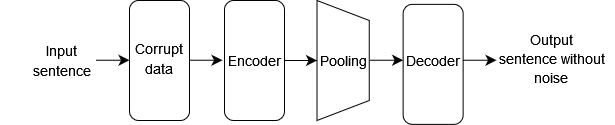
\includegraphics[width=\linewidth]{TSDAEdiagram.png}
	\caption{Architecture of TSDAE model}
	\label{fig:tsdae}
\end{figure}

For the purpose of classifying Slovenian sentences based on their sentiment we fine-tune the SBERT model with TSDAE. We choose bert-base-uncased (TODO) for our base model to fine-tune. For the loss function we use the DenoisingAutoEncoderLoss as our loss function when training. We train the method and compare our results with the corpus.


TSDAE has been shown by Wang, Reimers and Gurevych \cite{wang-etal-2021-tsdae-using} to outperform other unsupervised approaches and other supervised models, trained with a lot of labeled data. Many previous works were evaluated on Semantic Textual Similarity (STS) which might return good performance but it is unclear how it performs on specific domains. 


\subsection*{GPL}
GPL - opis metode, pri čemer se predvsem osredotočimo na domain adaptation. Povemo kateri model finetunamo.
Dodamo skico arhitekture.


\subsection*{Data}
Kakšne podatke uporabljamo, kako izgledajo, in what way did you prepare the data, delitev na množice (poudarimo, da se vse metode treniranjo z enako učno množico).
Pokažemo morda par primerov povedi v tabeli.


\subsection*{Testing approach}
Naslov morda še ni ustrezen in se bo prilagodil.
Katero metriko uporabimo za primerjavo rezultatov, kako iz sentence embedding pridemo do klasifikacije povedi.


%------------------------------------------------


\section*{Results}

TO DO:
Use the results section to present the final results of your work. Present the results in a objective and scientific fashion. Use visualisations to convey your results in a clear and efficient manner. When comparing results between various techniques use appropriate statistical methodology.


%------------------------------------------------

\section*{Discussion}

TO DO:
Use the Discussion section to objectively evaluate your work, do not just put praise on everything you did, be critical and exposes flaws and weaknesses of your solution. You can also explain what you would do differently if you would be able to start again and what upgrades could be done on the project in the future.


%------------------------------------------------

\section*{Acknowledgments}

Here you can thank other persons (advisors, colleagues ...) that contributed to the successful completion of your project.


%----------------------------------------------------------------------------------------
%	REFERENCE LIST
%----------------------------------------------------------------------------------------
\bibliographystyle{unsrt}
\bibliography{report}


\end{document}
